\begin{figure}[t]
  \UseAltLinespread
  \centering
  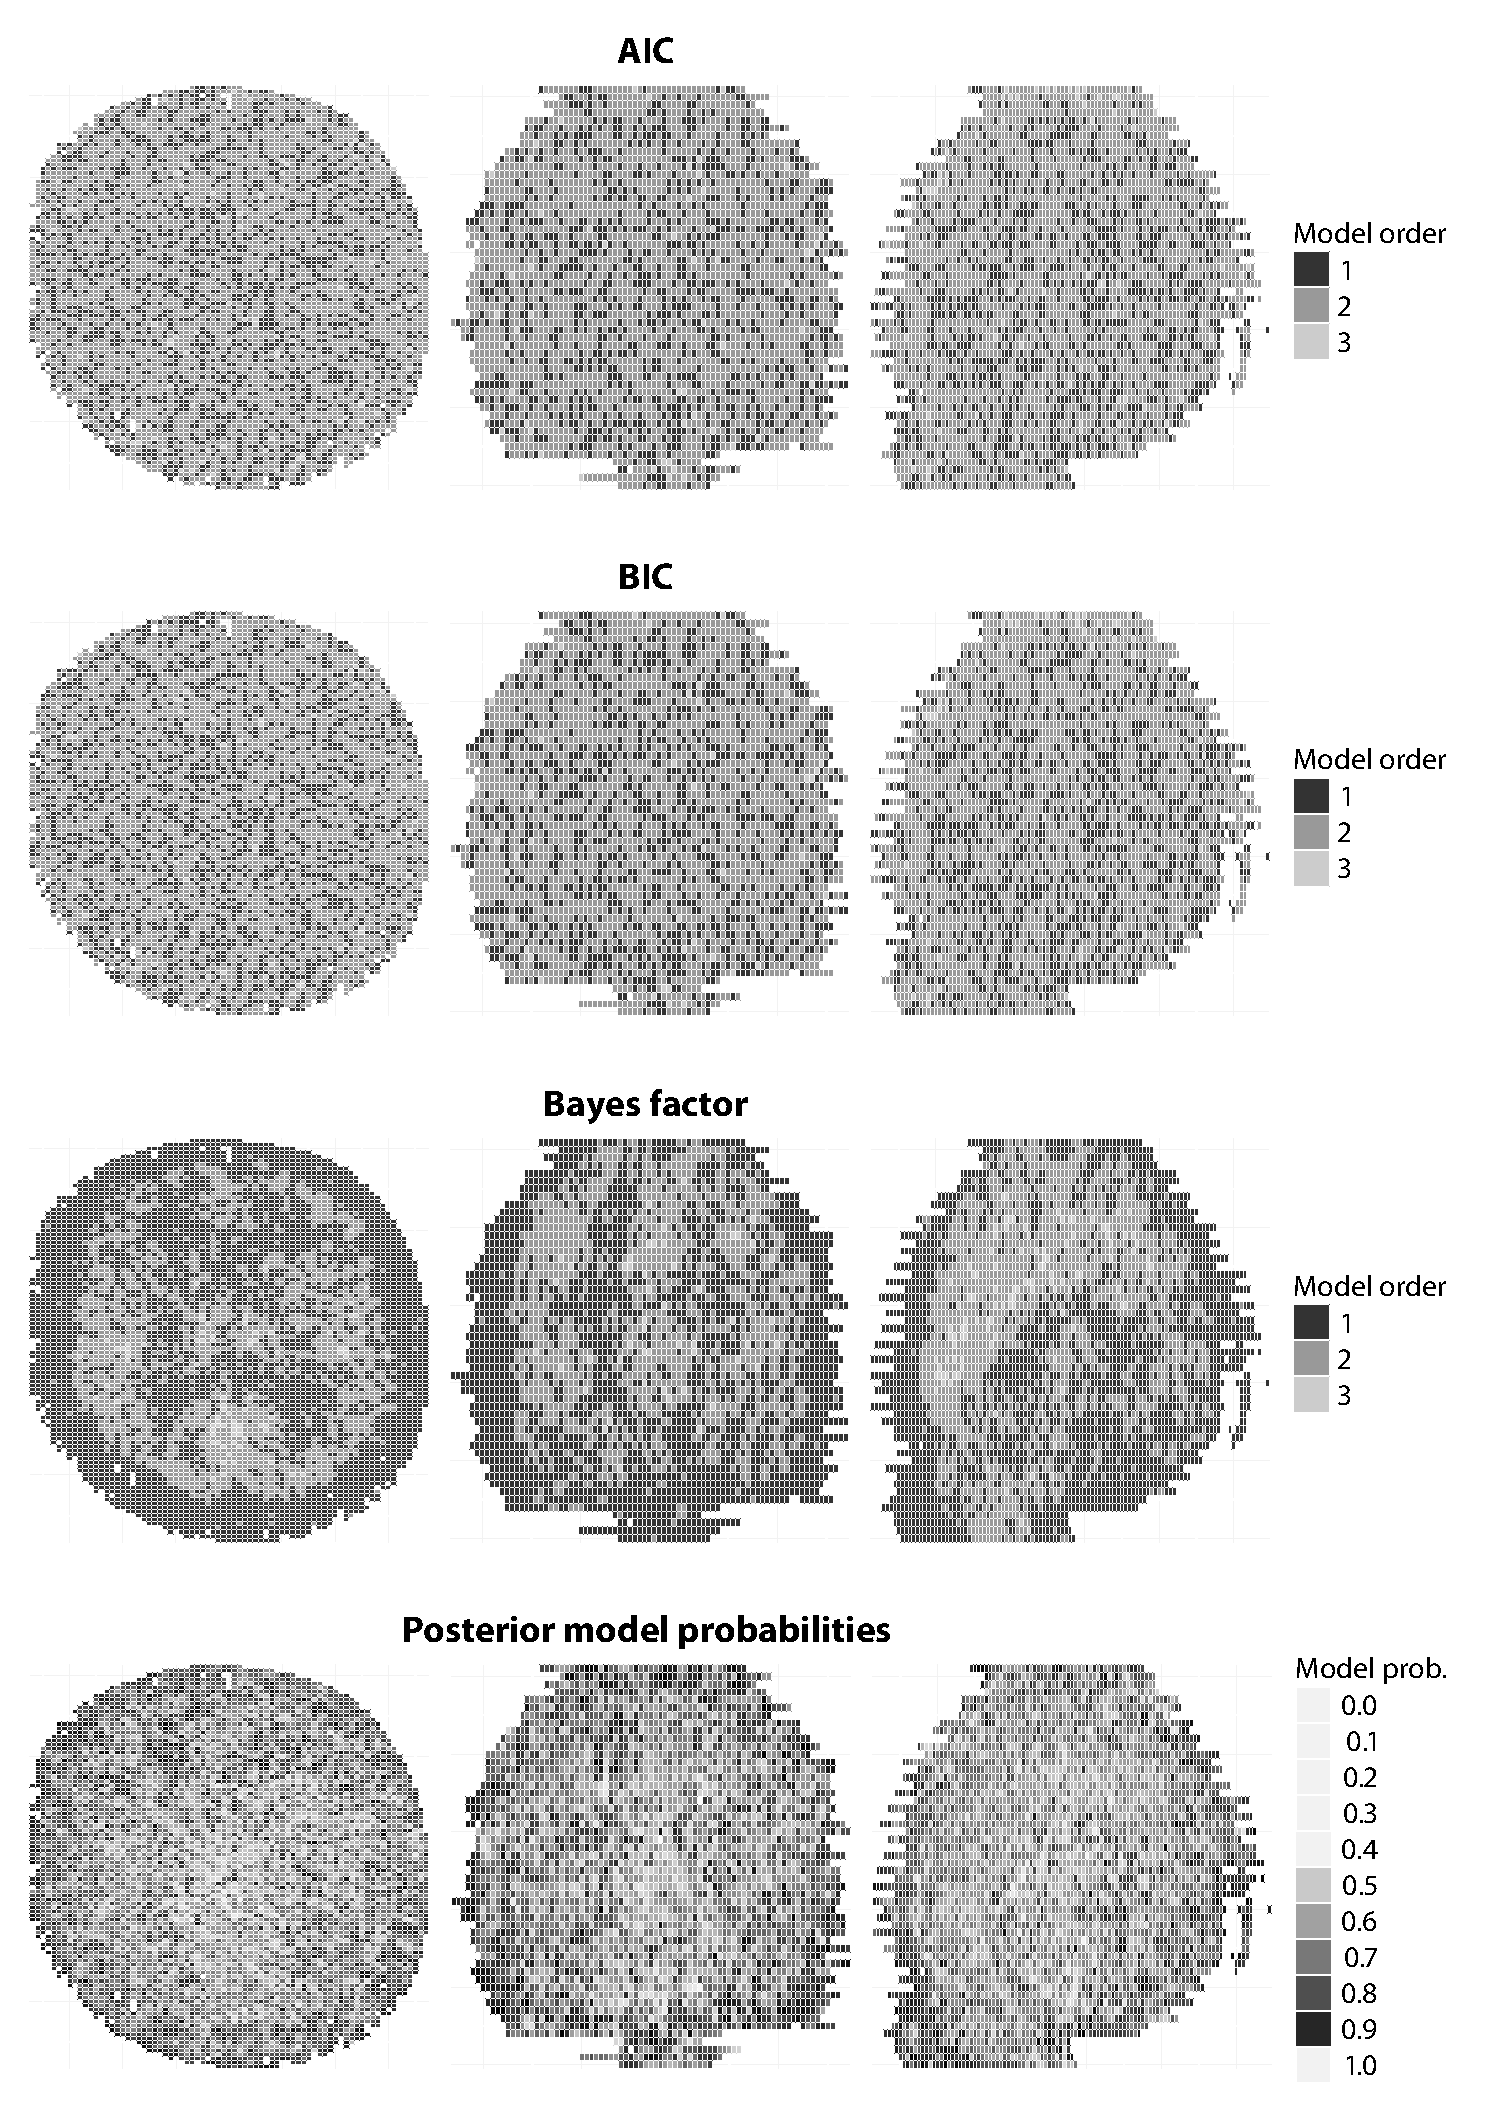
\includegraphics[width=0.95\linewidth]{fig_src/PET_MO}
  \caption[Model selection results for the \protect\pet compartmental model]
  {Model selection results for \pet model using real data set. In each row, three slice of the brain are shown in the plot. Each are close to the middle of the brain along each of the three axises in the three-dimensional space. From top to bottom: Model order selected by \aicc (see Section~\ref{sub:A second order aic}); Model order selected by \bic (see Section~\ref{sub:Bayes factor}); Model order selected by using Bayesian model comparison with marginal likelihood approximated by generalized harmonic mean estimator; The posterior model probability $\pi(\calM_k|\data)$ (see Section~\ref{sub:Model choice problems}) with uniform prior model probability $\pi(\calM_k)$.}
  \label{fig:pet mo}
\end{figure}
